\section{Introduction}\label{sec:introduction}

In recent years the Blockchain technology has rapidily emerged as a powerfull tool for supporting the development of many and innovative services and infrastructures. Blockchain-enabled applications are spreading across diverse sectors such as supply chain, business, healthcare, IoT, privacy, and data management \cite{blockchain_applications}. A blockchain is essentially a \textit{distributed ledger}, namely a database replicated across different locations and synchronized by multiple independent participants. Blockchains exploit the redundant, concurrent execution of the same transactions on a decentralized network of many machines, in order to enforce their execution in accordance with a set of predefined rules. Namely, blockchains make it hard, for a single machine, to disrupt the semantics of transactions or their ordering: a misbehaving single machine gets immediately put out of consensus and isolated. 
%
\begin{figure*}[th]
\centering
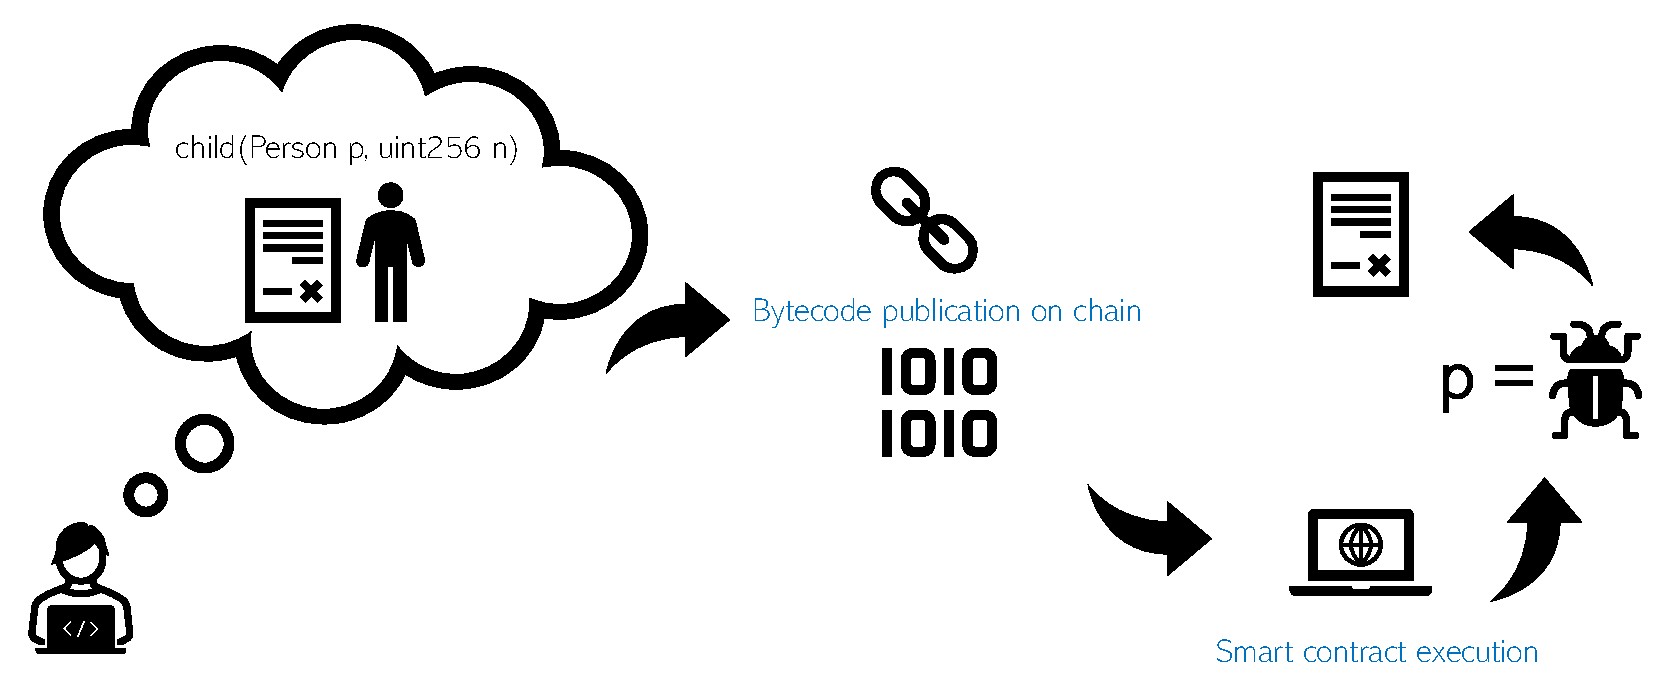
\includegraphics[width=0.8\linewidth]{figures/solidity_problem}
\caption{Example of possible problem that can occur in Solidity due to the absence of a strong typing mechanism.}
\label{figure.solidity_problem}
\end{figure*}
%
The key innovation introduced by this technology is a mechanism  able to reach an emergent agreement about a global state without the need for a central authority. Morever, another peculiarity is that the consensus is not explicit, because there is not a fixed moment when it occurs.

Bitcoin~\cite{Nakamoto08,book-mastering-bitcoin}  has been the first blockchain's success story. Here transactions are programmed in a non-Turing complete bytecode language, almost exclusively used to implement transfers of units of coins between \emph{accounts}, providing a totally decentralized P2P digital cash system based on a distributed public ledger. 
%
A few years after Bitcoin, another blockchain, called Ethereum~\cite{Buterin13,AntonopoulosW18}, introduced the possibility of programming transactions in an actual, imperative and Turing-complete programming language, called Solidity. The major innovation of Ethereum is the contrustruction through its nodes of a distributed \emph{world computer} that can run general purpose code. Indee, if the term ``distributed ledger'' is usually used to describe blockchains like Bitcoin, Ethereum is often defined as a ``distributed state machine''. Solidity's code is organized in \emph{smart contracts}, namely pieces of code which are stored in the blockchain and are executed when a particular event occurs, e.g. when a transaction is scheduled. From a theoretical point of view, a smart contract is essentially an agreement between two or more parties that can be automatically enforced without the need for a trustworthy intermediary~\cite{ebp}. Through smart contracts, Ethereum's transactions can hence execute much more than coin transfers. In this case the global shared state is given by a set of objects which are persisted and manipulated in the same way by all nodes in the blockchain through the execution of the same object constructors and methods.

The world computer built by Ethereum is known as Ethereum Virtual Machine (EVM) which is the platform where accounts and smart contracts live and are executed.
Solidity is high-level programming language and smart contracts need to be compiled into bytecode to be executed inside the EVM. At this regards, we can observe that in Solidity's bytecode, non-primitive values are referenced through a very general \<address> type. For instance, a Solidity method \<child(Person p, uint256 n) returns Person> actually compiles into \<child(address p, uint256 n) returns address>, losing most type information~\cite{CrafaPZ19}. Since, at run time, it is the bytecode that gets executed, everything can be passed for \<p>, not just a \<Person> instance, as illustrated in Fig.\,\ref{figure.solidity_problem}.
The compiler cannot even enforce strong typing by generating defensive type instance checks and casts, because values are unboxed in Ethereum: they have no attached type information at run time, they are just numerical \emph{addresses}. It follows that inside the \<child> method, an eventual call to a \<Person>'s method on \<p> might actually execute any arbitrary code, if \<p> is not a \<Person>. In other words, Solidity is not strongly typed. Consequently, it is highly discouraged, in Solidity, to call methods on parameters passed to another method, such as on \<p> passed to \<child>, since an attacker can pass crafted objects for \<p>, with arbitrary implementations for their methods, which can result in the unexpected execution of dangerous code. This actually happened in the case of the infamous DAO hack~\cite{dao16}, that costed millions of dollars.

Strong typing is one of the reasons that push towards the adoption
of \emph{traditional} programming languages for smart contracts. For instance,
the Cosmos blockchain~\cite{cosmos} uses Go. The
Hotmoka blockchain~\cite{hotmoka} uses a subset of Java
for smart contracts, called Takamaka~\cite{Spoto19,Spoto20}.
Hyperledger~\cite{hyperldeger} allows Go and Java.
Another reason is the availability of modern
language features, that are missing in Solidity,
such as \emph{generics}\ie the possibility of using
type variables. Generics are a powerful and very useful facility for programming
smart contracts, since they allow one to personalize the behaviour of such contracts and partially overcome their inherent incompleteness~\cite{ebp}. 
%
Through the use of generics, it is possible to provide to users a set of predefined contract templates which can be extended and specialized by users with lower programming skills, but higher knowledge about the specific application domain. They are based on the use of type placeholders in order
to produce parametrized code, that can be instantiated for each
concrete type provided for the placeholders.
%
However, strong typing and generics are two intertwined language features that have to be carefully considered when smart contracts are implemented and their bytecode is subsequently deployed on a blockchain. For instance, in Java source code, generics are strongly typed, if no \emph{unchecked operations} are used~\cite{NaftalinW06}, as it will always be the case in this paper.
However, generics might have security issues at the level of compiled Java code and this paper originated from a real issue that we found in our code.



The contribution of this paper is to show a real-life
use of generics for an actual smart contract contained in the support
library of the Takamaka language, and to demonstrate that a na\"{i}ve use
of Java generics can lead to a code security vulnerability that
allows an attacker to earn money by exploiting someone else's work, with both economical and legal side effects.
This paper will provide a fix to that specific issue,
by proposing a re-engineering of the code that forces the compiler to generate defensive checks.
More generally, this paper can be useful for the definition of
bytecode languages for future smart contract languages, by
learning from the weaknesses of Java bytecode.

The remainder of this paper is organized as follows.
Sec.~\ref{sec:java_generics} discusses the management of generics in Java.
Sec.~\ref{sec:takamaka} presents the basic notions about the Takamaka language for smart contracts in Java.
Sec.~\ref{sec:shared_entities} shows our real-life Java smart
contracts for shared entities, that use generic types.
Sec.~\ref{sec:validators} shows the instantiation of the shared entities to implement the validators' set
of a proof of stake blockchain.
Sec.~\ref{sec:attack} shows that a na\"{i}ve
deployment of a subclass of the validators' set leads to a code vulnerability.
Sec.~\ref{sec:fix} presents a fix to that vulnerability.
Sec.~\ref{sec:related_work} discusses some related work.
Sec.~\ref{sec:conclusion} concludes.

This paper is a revised and extended version of~\cite{BeniniGMS21}.
In comparison to that paper, Sec.~\ref{sec:takamaka} and
Sec.~\ref{sec:validators} are new; while all other sections have been expanded and the enriched with several explanatory figures.
